\chapter{Data fusion in the Kalman module}
\section{Initial Matlab Parameter Simulation}
Before starting development for the robot, the beginning of the project was spent on building a simple \textsc{Matlab} simulation of a Kalman Filter.
This allowed the group to get acquainted to the different parameters of a Kalman Filter and to learn how they influence estimation.

By inserting velocity data and analyzing the predictions we gained much insight into the Kalman Filter model. Additionally the effects of the noise covariances became much clearer in a way that was very helpful throughout the project.

\section{ROS Package Dependencies}
\subsection{Robot localization}
For the functionality of the Kalman Filter the package \texttt{robot\_localization} is used. The package provides a convenient 15-dimensional implementation of the Kalman Filter with direct support for 6D pose, 6D velocity and 3D acceleration vectors. The available inputs can be dynamically configured in the \texttt{.launch} file for the \texttt{robot\_localization} node. In general the whole package is configurable via \texttt{.launch} file or \texttt{.yaml} file.

\subsection{TF (Transformation)}
The \texttt{TF} package is used to define all sorts of data transformations in different coordinate systems. In this case the robot's map data and the input of the marker detection are converted to be fused in a common coordinate system. 

\section{Package Structure / Design}
The Kalman package consists of three sub-packages two of which are used for development purposes. They are described in detail in the following sections:
\begin{description}
\item[\texttt{sensor\_dummy:}] Placeholder nodes used to generate artificial sensor data.
\item[\texttt{kalman\_debug:}] A package for visual monitoring and evaluation.
\item[\texttt{kalman\_global:}] The production package that performs input conversions and publishes estimates.
\end{description}

The package is designed to be highly dynamic. All properties and settings can be configured by \texttt{.yaml} files and \texttt{.launch} files similar to the \texttt{robot\_localization} package. So no recompilation is required if new topic names are chosen or the resulting frames of the data change.

\subsection{package \texttt{kalman\_global}}
This package contains the actual logic for data fusion.

\subsubsection{Parameter overview}
For full flexibility \texttt{kalman\_global} defines namespaces containing names for all parameters that are configurable through \texttt{yaml} files at runtime. For example the \texttt{node} namespace includes following parameters:
\begin{description}
\item[converter] Node for converting poses into appropriate frames.
\item[ekf\_launch] Launch file for the Extended Kalman Filter (EKF) from \texttt{robot\_localization}.
\item[set\_pose] This node tests the pose reset functionality in case of a kidnapping.
\item[visualizer] The visual monitoring and debugging node using rviz.
\end{description}

Several IDs are listed in the \texttt{param} namespace: world, map, odom, frame and base link id. It also contains all service as well as topic names that the package listens on or publishes to:

\begin{description}
\item[``/vision/estimated\_pose''] Derived poses from the Kinect arrive here in \textbf{global frame}.
\item[``/poseupdate''] The converter listens on this topic to receive poses from laser sensors in \textbf{local\_map frame}. 
\item[``laserProcessed''] The laser pose is converted to the same frame as the Kinect frame (\textbf{global}) and re-published here for the EKF.
\item[``/odometry/filtered''] The EKF publishes its filtered pose here in \textbf{local\_map}.
\item[``fused\_pose''] After the filtered data is converted to \textbf{world frame}, it is re-published here as final output.
\item[``/HL/is\_kidnapped''] The high level module publishes a flag on this topic whenever the kidnapping state changes.
\item[``reset\_sensor\_srv''] Whenever the robot has recovered from kidnapped state this service can optionally be called to feed the position from kidnap recovery  into an artificial \textit{reset sensor} with very low covariances.
\item[``reset\_sensor''] The reset position from above service is published to the EKF on this topic.
\end{description}

\subsubsection{Robot Localization Node (EKF)}
\begin{description}
\item[Subscriptions]\
\begin{itemize}
	\item ``laserProcessed''
	\item``/robot/lauron/odom''
	\item ``/vision/estimated\_pose''
	 \item ``reset\_sensor'' 
\end{itemize}
	
\item[Publications]\
	\begin{itemize}
	\item ``odometry/filtered''
	\end{itemize}
\end{description}

This node is part of the ROS \texttt{robot\_localization} package and implements the \textit{Extended Kalman Filter} (EKF). An \texttt{ekf\_params.yaml} file configures it by defining initial estimate covariance, process noise covariances, queue sizes, publishing frequency and subscripted topics.

It listens on the `laserProcessed'' topic to which the converter publishes laser data that is converted from local\_map to global frame. This is fused with the robot's odometry data from \\ ``/robot/lauron/odom'' topic and ``/vision/estimated\_pose'' to which the vision module publishes poses derived from camera images.

It is also subscripted to ``reset\_sensor''. Here a new position with very low covariances is optionally published to convince the filter to trust the pose obtained on kidnap recovery. Although this can be used to correctly reset the filter, another approach is currently active, see TODO.

Finally, the fused pose is published to \textbf{``odometry/filtered''} in local\_map.

\subsubsection{Converter Node}
\begin{description}
\item[Subscriptions]\
	\begin{itemize}
	\item ``/vision/estimated\_pose'' 
	\item ``/poseupdate'' 
	\item ``odometry/filtered'' 
	\item ``/HL/is\_kidnapped'' (optional)
	\end{itemize}
	
\item[Publications]\
	\begin{itemize}
	\item ``laserProcessed''
	\item ``fused\_pose''
	\end{itemize}
\end{description}

The converter node has two tasks:

\begin{enumerate}
\item Transform sensor poses into a uniform frame for the EKF (global).
\item Transform the EKF result into frame usable by the other modules (world)
\end{enumerate}

Specifically it transforms laser input into the same frame as the pose from the vision module (global), then publishes it on ``laserProcessed'' for the EKF.

It then listens on the EKF's result topic ``odometry/filtered'' to transform the filtered local\_map pose into world frame. This transformed result is published to ``fused\_pose'' and is used by the other modules as final pose estimation. Figure \ref{ekf - converter} summarizes interaction between converter and EKF.

\begin{figure}[ht]
\centering
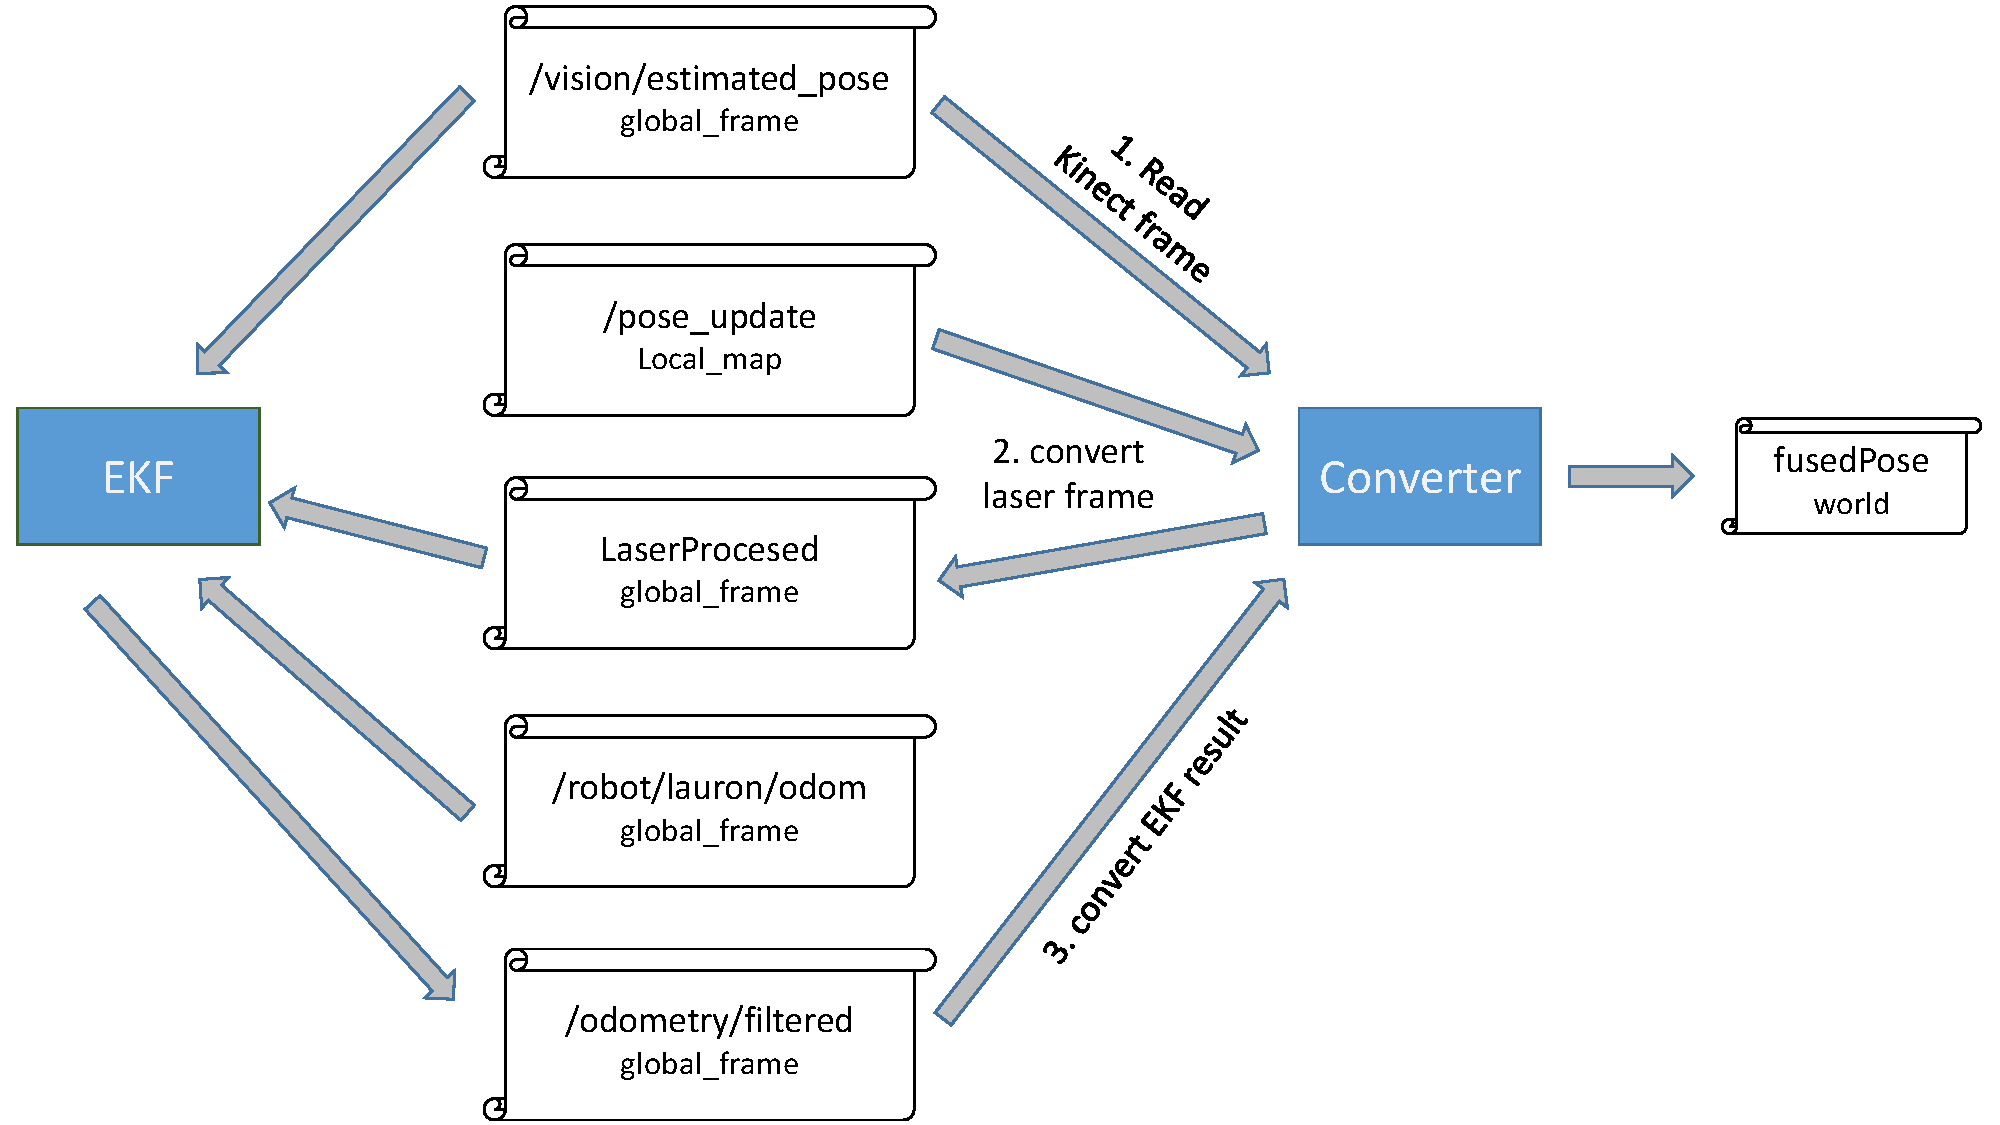
\includegraphics[width=\textwidth]{graphics/ekf_converter.pdf}
\caption[EKF -- Converter interaction]{Interaction between EKF and Converter: The converter transforms laser data and EKF output into desired frames.}
\centering
\label{ekf - converter}
\end{figure}


\subsubsection{set\_pose node -- kidnap reset}
\begin{description}
\item[Owns service] ``reset\_sensor\_srv''
\item[Publications] ``reset\_sensor\_service''
\end{description}

This optional node can be called from high level module to force a new pose in case of a kidnapping.

As soon as the robot recognizes a marker, it recovers from kidnapped state and a call to ``reset\_sensor\_srv'' is made with a position derived from the marker.

The new position is in turn published to ``reset\_sensor\_service'' with an artificially low covariance so that it will be accepted as new pose by the EKF.

\subsection{package \texttt{sensor\_dummy}}
In the first months of the project it was impossible to test implementation with real input since all teams started from scratch. Production and publication of sensor data was just being developed. To overcome this obstacle, artificial test data was generated and used as output of placeholder sensor nodes. 

Test data from two different generation techniques have been employed: a quick but very unrealistic solution in \textsc{Matlab} and later a more sophisticated simulation using the MonoGame framework.

\subsection{Test data from \textsc{Matlab}}
In \textsc{Matlab} test data was generated by supplying a number of points provided by the user and distributed over time. The \textsc{Matlab} script uses a cubic spline interpolation to generate the values in between. For simplicity these values were initially only generated for one dimension of the Kalman Filter.

Primitive testing was possible with this data virtually from day one.

\subsection{Simple MonoGame}
For the generation of more realistic test data, including 2D poses and robot view angle, a small \texttt{C\#}-program was built. This program uses the MonoGame framework to allow mouse interaction in a window. A small arrow is displayed to represent the robot. Then by clicking on a position the user can tell the robot to move there with a pre-defined fixed speed. When holding down the mouse button and releasing it on another pixel the vector between these points is used to generate the target view angle of the robot. In the background the program continuously writes the current position and view angle to a file.

\subsection{Sensor Test Data Dummy node}
\begin{description}
\item[Publications]\
	\begin{itemize}
	\item ``/poseupdate''
	\item ``/vision/estimated\_pose''
	\end{itemize}
\end{description}

Two placeholder sensor nodes -- representing laser sensor and Kinect -- read from the test data files and published them in a loop on ``/poseupdate'' (laser topic) and ``/vision/estimated\_pose'' (Kinect topic).

This way the Kalman Filter could be tested even if the actual sensor nodes were still in development. It was now possible to tweak the many parameters of the \texttt{robot\_localization node} and study the filters behavior independently of the other groups.

\subsection{Package \texttt{kalman\_debug}}
After development of the input and procesing pipeline for test data, the next challenge was to evaluate the filter's outputs. Since it is very difficult to interpret the fused poses by only looking at numbers, the ROS package \texttt{rviz} was utilized to visually compare input data and filtered result.

The visual proof for the effects of parameter changes greatly enhanced our capability to evaluate the Kalman filter's performance. In the figures \ref{Fig: Kalman Fusion - Low}, \ref{Fig: Kalman Fusion - Medium} and \ref{Fig: Kalman Fusion - High} the change of the target position's x component over time is visualized. The \textbf{blue line} represents the position received from ``/vision/estimated\_pose'' while the \textbf{red line} represents the data received from ``laserProcessed''. The \textbf{green line} is the fused data of the kalman filter read from ``fused\_pose''.

\subsection{visualizer node}
\begin{description}
\item[Subscriptions]\
	\begin{itemize}
	\item ``/vision/estimated\_pose'' 
	\item ``laserProcessed''
	\item ``fused\_pose''
	\end{itemize}
	
\item[Publications]\
	\begin{itemize}
	\item ``visualization\_marker''
	\end{itemize}
\end{description}

The visualizer node subscribes to the output topic of the Kalman Filter (``fused\_pose'') and the sensor topics ``laserProcessed'' and ``laserProcessed'' to create displayable markers that can be used to evaluate data fusion quality. These displayable markers are of type \\ \texttt{visualization\_msgs::Marker} and published to the ``visualization\_marker'' topic on which \textit{rviz} is subscripted. The received markers appear in the rviz coordinate system as they arrive.

There are two possible visualization modes:

\begin{itemize}
\item Show the current 2D pose of each marker.
\item Show change over time of pose in x for each marker.
\end{itemize}

It might also be useful to display process covariances over time to gain a better understanding of why there is a sudden change in the kalman filter's behavior.

\subsection{set\_pose node}
\begin{description}
\item[Client to service] ``reset\_sensor\_srv''
\end{description}
This node tests pose reset in kidnapping situations. It calls the ``reset\_sensor\_srv'' service with a a dummy pose to overwrite the current pose.

The effect of this call can be viewed in rviz where the fused pose's marker is expected to jump to the new pose. In figures \ref{Fig: Kalman Fusion - Low}, \ref{Fig: Kalman Fusion - Medium} and \ref{Fig: Kalman Fusion - High} this behavior is shown by displaying the position's x component over time. As before the \textbf{blue line} represents the position received from ``/vision/estimated\_pose'', the \textbf{red line} represents data received from ``laserProcessed'' and the \textbf{green line} is fused data of the kalman filter read from ``fused\_pose''.

In the tests camera and laser pose estimation are artificially chosen wide apart. The behavior of the kalman filter is shown if the input stream of ``laserProcessed'' stops for a while and starts sending again.

As can be seen, the amount of time to jump back to normal pose increases with higher system confidence.

\begin{figure}[thpb]
      \centering
      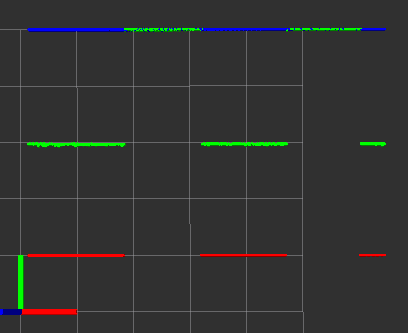
\includegraphics[width=0.5\textwidth]{graphics/kalman_fast.png}
      %\includegraphics[scale=1.0]{figurefile}
      \caption{Kalman fusion - low system confidence}
      \label{Fig: Kalman Fusion - Low}
   \end{figure}

\begin{figure}[thpb]
      \centering
      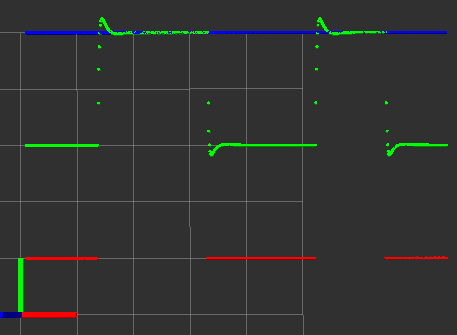
\includegraphics[width=0.5\textwidth]{graphics/kalman_medium.png}
      %\includegraphics[scale=1.0]{figurefile}
      \caption{Kalman fusion - medium system confidence}
      \label{Fig: Kalman Fusion - Medium}
   \end{figure}
	
\begin{figure}[thpb]
      \centering
      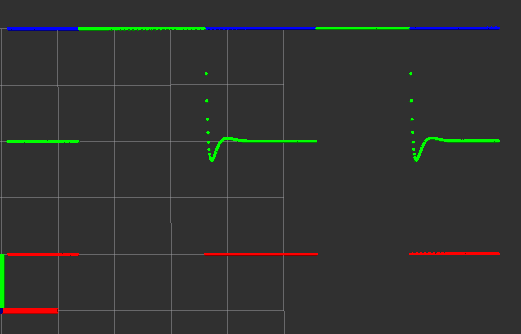
\includegraphics[width=0.5\textwidth]{graphics/kalman_slow.png}
      %\includegraphics[scale=1.0]{figurefile}
      \caption{Kalman fusion - high system confidence}
      \label{Fig: Kalman Fusion - High}
   \end{figure}

\section{Difficulties}
\subsection{Initial start with custom Kalman Implementation}
Before using the \texttt{robot\_localization} package a quick attempt to implement the Kalman Filter manually was investigated. Luckily our attention was directed towards the \texttt{robot\_localization} package before more than data subscription and publishing were implemented, both of which were fortunately reused throughout the project.

\subsection{Difficulties with employing MCA2}
When the Kalman Filter performed satisfactorily with the artificial test data, the next step consisted of producing more realistic data with a true robot simulator. For this MCA2 appeared to be a suitable solution. But the installation of MCA2 and the simulator presented unexpected difficulties and failed in the end.

One of the reasons is the quality of the MCA2 documentation which posed a major problem. It is highly fragmented, redundant, often outdated and in some places contradictory. Very often it was difficult to understand if an installation error was caused by a user mistake or by the documentation and if the latter, whether it is only unclear, incomplete or incorrect. 

The usual approach for a computer scientist is to read the documentation and rule out any self-made errors before asking possibly unnecessary questions. This is why the lacking documentation caused more harm than good.

It was finally discovered that additional data only existing on a USB drive was required in order for the package to install successfully. But even after having received this piece of data the software could only be run exclusively on lab computers, indicating another still unknown dependency or requirement.

By that time data publishing and necessary software for it have already been facilitated on the robot. So MCA2 was abandoned and the robot itself was used to generate data.

\subsection{Roslaunch initialization and ROS\_IP behind NATs}
While working with virtual machines for ROS package development the problem of incorrect communication between the packages was discovered. Only when starting the nodes in the right order with appropriate delays in between, the system would work on the robot. In general the specification of the \texttt{ROS\_IP} environment variable is used to solve that issue. The local IP of the virtual machines behind a NAT was not available and so the execution of the nodes was completely moved to the robot.

\subsection{Boundary for accepted jumps between sensor outputs}
When first configuring the \texttt{robot\_localization} package, a threshold for tolerated jumps in the sensor data was set to a rather low value. This caused the Kalman Filter to exhibit a lot of unexpected behavior, for instance it did not respect changes in one sensor at all. After setting the threshold to an appropriate value, the filter worked even better as initially expected. This is partly due to the well adjusted remaining parameters of the Kalman Filter which were already thoroughly tested with the Matlab simulation.

\subsection{Set pose of robot\_localization does not work as expected}
The \texttt{robot\_localization} package provides a \texttt{set\_pose} topic to force the actual pose of the robot. It was planned to use this topic to inform the Kalman Filter about the new pose after having recovered the robot from kidnapped state. Unfortunately this sets the pose permanently and further input is ignored, so another solution was necessary.

The approach of choice uses a third virtual input sensor that sends the recovered pose along with very low covariances to convince the Kalman Filter to trust this source the most.

But in the final implementation the necessity to react to a kidnap event was disabled in the Kalman filter. Instead, we opted for a simpler behaviour: the high level logic updates the transform immediately after having resolved the kidnapping, so that sensor data discrepancies are removed. 

\subsection{Unclear information about the data source topics and types for the data fusion}
Finding out which scripts must be started on the robot to make it publish its pose and twist turned out to be a challenge in itself. During some periods alternative topics were used to at least receive any data to work with. For example the map position of the robot was temporarily replaced by its odometry output.